\section{Sample Time}
\label{ch:performance-sampletime}
%A bottleneck on the accuracy of the final image is the amount of error introduced by the sampling of the velocity profile produced by the solution of the time-optimal control problem. Sampling error is an unavoidable result of a digital system following a given profile. Thus there is a limit on the accuracy of a digital system, especially one which uses integration in order to achieve an outcome. The smallest amount of error will magnify until the result is quite different from that which is desired. Since a digital processing device can only direct an integrating process at a limited rate, sampling errors will accumulate over time and cause the image to become inaccurate. In the case of the DoodleBot, the measured placement of the initial position at the initialisation of a trajectory resets the integration error and as such the error can only accumulate over a single curve. The effect of operating at differing sample periods can be seen in Figure \ref{fig:timestep}.

The Optimisation module is able to produce continuous velocity profiles that perfectly track the required URBS, however the PLC and network interface require discrete sampled packets, and so the velocity profiles need to be discretized. This is inherently an approximation that will lose accuracy.
\begin{figure}[hp]
\includegraphics[width=\textwidth]{figures/performance/timestep.png}
\caption[Comparison of differing velocity sampling frequencies]{A comparison of velocity sampling periods. From top left to bottom right; 1) 20ms 2) 40ms 3) 80ms 4) 120ms 5) 150ms 6) 200ms
\label{fig:timestep}}
\end{figure} 

\begin{figure}
\centering
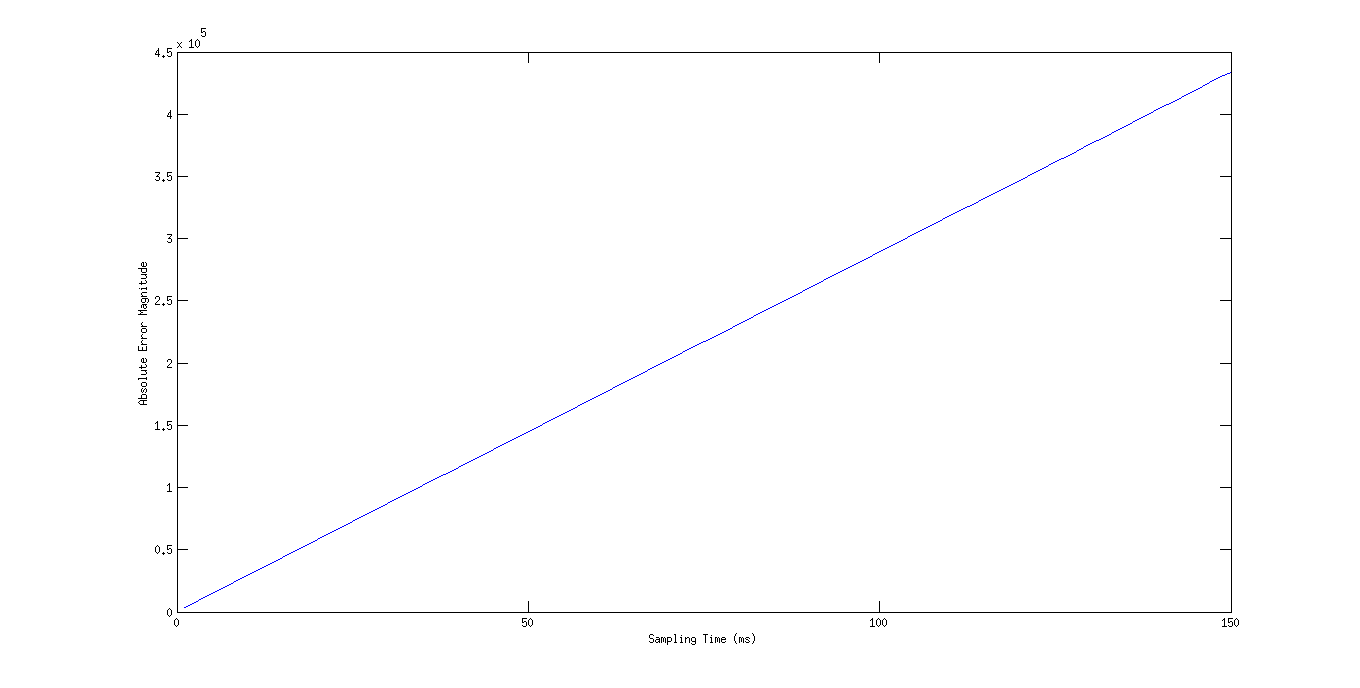
\includegraphics[width=0.8\textwidth]{figures/performance/tStep.png}
\caption[Plot of error magnitude against velocity sampling period]{Error magnitude against velocity sampling period, where the error is calculated to be the distance between the original curve and the sampled curve}
\label{fig:tStep}
\end{figure}  

Figure ~\ref{fig:tStep} shows a chart of the error in the image verses the sampling time, where the error is the deviation between the sampled curve and the original curve summed for a certain number of samples across the length of the curve. The chart shows that as the sampling time drops  the error reduces linearly.

However in the real system, there are minimum constraints on how low the sampling period can go. The sample rate cannot be lower than the time it takes for the network interface to buffer more commands and it cannot be lower than the time it takes for the PLC to process the command and then implement it on the stepper motors, or whole commands will be skipped. 

Another major effect of lower sampling rates becomes apparent in Figure ~\ref{fig:timestep}. As the sample time reduces from 200ms to 40ms, there is a clear improvement in the accuracy of the image, as the simulated results would suggest. However, when the sampling time is reduced to 20ms the error actually increases significantly. 

\begin{center}
\centering
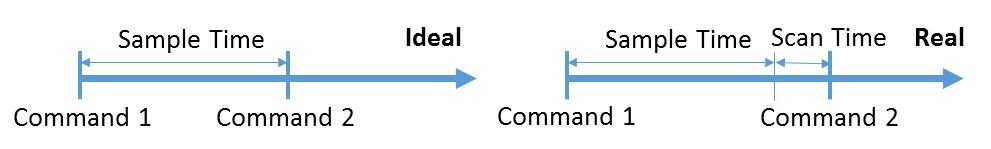
\includegraphics[width=0.6\textwidth]{figures/performance/images/periodscan.jpg}
\captionof{figure}[Sample time inaccuracy]{Real vs ideal behaviour of PLC code sample time}
\label{fig:periodscan}
\end{center}

This unexpected error with lower sample times is likely due to how accurately the PLC is actually able to operate at the specified sample time. Figure ~\ref{fig:periodscan} shows a real vs ideal scenario on how sample time can vary. In the ideal scenario, as soon as the internal counter reaches the sample time a command will be executed and the timer reset. In reality, the PLC has to scan through the code one line at a time and might take some extra time before executing the command and resetting the internal timer. This means that the system will run a single command for longer than it should. 

The PLC scan times vary from 0.1ms-1.5ms, and hence cannot be compensated for in the code. Since the scan times don't seem to be effected by sample times, lower sample times lead to a higher proportional error in the real vs specified sample time. This creates a trade off between inherent error from approximation by lowering the scan times and minimizing the proportion of error between the real and ideal scan times by increasing the scan times. Experimentation found $40ms$ or $25Hz$ to be the best compromise between these two trade offs. 



 



%Two effects are at play in the alteration of the sampling period. A limit exists on the lowering of the sampling period below the time required for the controller to undergo one iteration of the control loop. Beyond this point variance in the loop timing can weight some commands noticeably more than others, even to the point where commands begin to get skipped or are not active for a long enough duration to have an effect. This causes the type of distortion in the final image that can be seen in the top left profile in Figure \ref{fig:timestep}. The second effect of the sampling period on the accuracy of the output image is that an increase in the sampling period corresponds to a larger approximation of the correct velocity profile. The looser an approximation becomes, the greater the integral error will become over the length of the curve. Figure \ref{fig:timestep} demonstrates this effect. As the as the sampling period increases the amount of error becomes progressively greater. Figure \ref{fig:tStep} demonstrates that the level of error in the final image is linearly correlated with respect to the sampling period.

%It is evident that the best policy is to decrease the sample period until just before the limits of the control loop manifest. The DoodleBot was found to perform best at a 40ms sampling period, or at 25Hz.